\documentclass[aspectratio=169,12pt]{beamer}
\usepackage{tikz}
\usetikzlibrary{arrows.meta, positioning}

\usepackage{polyglossia} % Translation
     \setdefaultlanguage{spanish}
\usepackage{fontspec} % New Fonts and stuff
\usepackage{xstring} % Command/Envs Args Strings Handling
\usepackage{ragged2e} % Text align
\usepackage{graphicx} % Images
\usepackage[labelfont={color=unalDk2}]{caption} % Images, figures and graphics caption config
\usepackage{tcolorbox} % Color Box
\usepackage{enumitem} % Enumerate and Itemize styling
\usepackage{biblatex} % bibliography

\usepackage{mathtools} % Math macros, commands and stuff
\usepackage{unicode-math} % Math text

% ============================================================
% — Esquema UNAL 2024 — Tema VERDE
% ============================================================
%  Extraídos de theme1.xml del archivo verde .pptx
%
%  Mapeo de roles (diferencias respecto al tema morado):
%  unalAcc1  →  accent3  #06784F  verde oscuro  (títulos, líneas)
%  unalAcc5  →  accent4  #14C486  verde claro   (numeración listas)
%  unalDk2   →  #06784F  verde oscuro (pie de página)
%
%  Colores compartidos con el tema morado:
%  unalDk1   #29272D  texto oscuro
%  unalLt1   #F7F5F2  fondo claro
%  unalBg2   #F7F5F2  texto sobre fondos oscuros
%  unalAcc2  #FFB93E  amarillo (líneas decorativas del fondo)

\definecolor{unalDk1}  {HTML}{29272D}
\definecolor{unalLt1}  {HTML}{F7F5F2}
\definecolor{unalDk2}  {HTML}{06784F}   % verde oscuro — pie de página
\definecolor{unalLt2}  {HTML}{F8ECCD}
\definecolor{unalAcc1} {HTML}{06784F}   % verde oscuro — títulos, líneas
\definecolor{unalAcc2} {HTML}{FFB93E}   % amarillo
\definecolor{unalAcc3} {HTML}{06784F}   % verde oscuro
\definecolor{unalAcc4} {HTML}{14C486}   % verde claro
\definecolor{unalAcc5} {HTML}{14C486}   % verde claro — numeración listas
\definecolor{unalAcc6} {HTML}{F79646}   % naranja
\definecolor{unalBg2}  {HTML}{F7F5F2}   % crema/blanco


% Información constante en la presentación

% --- Información institucional ---
\newcommand{\Facultad}{Ciencias}
\newcommand{\Sede}{Bogotá}
\newcommand{\Departamento}{Matemáticas}

% --- Información presentación ---
% Lo mejor es redefinirlas en el main.tex
\newcommand{\Titulo}{Closure-Class Semantics for Keys and Normal Forms in Relational Schema Analysis} 
\newcommand{\Subtitulo}{Revición Estructural}


% New Fonts
% Ancizar parece ser el estandard de las presentaciones en la UNAL

\newfontfamily\AncizarSerif{AncizarSerif-Regular}[
    Path=config/src/font/,
    Extension=.ttf
]
\newfontfamily\AncizarSerifEB{AncizarSerif-ExtraBold}[
    Path=config/src/font/,
    Extension=.ttf
]

\newfontfamily\AncizarSans{AncizarSans-Regular}[
    Path=config/src/font/,
    Extension=.ttf,
]
\newfontfamily\AncizarSansEB{AncizarSans-ExtraBold}[
    Path=config/src/font/,
    Extension=.ttf
]
\newfontfamily\AncizarSansLight{AncizarSans-Light}[
    Path=config/src/font/,
    Extension=.ttf
]
\newfontfamily\AncizarSansItalic{AncizarSans-Italic}[
    Path=config/src/font/,
    Extension=.ttf
]

% Default Fonts
\setmainfont{AncizarSans-Regular}[
    Path=config/src/font/,
    Extension=.ttf,
    BoldFont=AncizarSans-ExtraBold,
    ItalicFont=AncizarSans-Italic,
    SmallCapsFont=AncizarSans-Light,
]
\setsansfont{AncizarSans-Regular}[
    Path=config/src/font/,
    Extension=.ttf,
    BoldFont=AncizarSans-ExtraBold,
    ItalicFont=AncizarSans-Italic,
    SmallCapsFont=AncizarSans-Light,
]


% Configuraciones generales de Beamer, la template y otros...

% Quita los controles default de Beamer
\setbeamertemplate{navigation symbols}{}

% --- Colores beamer ---
\setbeamercolor{normal text}      {fg=unalDk1}
\setbeamercolor{background canvas}{bg=white}
\setbeamercolor{itemize item}     {fg=unalAcc5}
\setbeamercolor{enumerate item}   {fg=unalAcc5}
\setbeamercolor{footlinecolor}    {fg=unalBg2,bg=unalAcc1}

\setbeamertemplate{itemize item}  {\textcolor{unalAcc5}{\textbullet}}
\setbeamertemplate{enumerate item}{\textcolor{unalAcc5}{\insertenumlabel.}}

% --- Headline (base) ---
% Los espacios de margen de las lineas son aprox. 3.5% horizontalmente y 5% verticalmente.
% El tamaño del 'bloque' al final de la línea aprox. 19% horizontalmente y 1.5% verticalmente.
% Según las imágenes de 'referencia' de la plantilla
\setbeamertemplate{headline}
{%
    \vspace*{0.03\paperheight}
    \hspace*{0.035\paperwidth}\makebox[\textwidth][l]{\color{unalAcc1}\AncizarSansLight\fontsize{10pt}{12pt}\insertslidenumber{}}
    \hspace*{0.035\paperwidth}{\color{unalAcc2} \rule[-0.01\paperheight]{0.93\paperwidth}{0.7pt}}
    \hspace*{0.775\paperwidth}{\color{unalAcc2} \rule{0.19\paperwidth}{0.013\paperheight}}
}

% --- Footline ---
% El tamaño del pie de linea aprox. 10.8% de altura.
\setbeamertemplate{footline}
{%
    \begin{beamercolorbox}[wd=\paperwidth,ht=0.08\paperheight]{footlinecolor}
        \begin{columns}
            \begin{column}{0.7\paperwidth}
                {\AncizarSansItalic{\fontsize{10pt}{12pt}{Facultad de \Facultad}}}\\
                {\AncizarSansItalic{\fontsize{10pt}{12pt}{Sede \Sede}}}
                \vspace*{5pt}
            \end{column}
            \begin{column}{0.1\paperwidth}
                bye
            \end{column}
        \end{columns}
    \end{beamercolorbox}
}

% --- Title / Subtitle ---
\setbeamertemplate{frametitle}
{%
    \vspace*{-0.02\paperheight}
    \fontsize{18pt}{20pt}
    {\color{unalAcc1} \AncizarSerifEB{\insertframetitle{}}} \\
    \fontsize{10pt}{12pt}
    {\color{unalAcc1} \AncizarSansLight{\MakeUppercase{\insertframesubtitle{}}}}
}


% Slides predefinidas de la template

\NewDocumentCommand{\SlideFrontCover}{}
{{%
    \setbeamercolor{background canvas}{bg=unalAcc1}
    \setbeamertemplate{headline}
    {%
        \vspace*{0.025\paperheight}
        \fontsize{8pt}{12pt}
        \makebox[\textwidth][l]{\color{unalAcc1}\AncizarSansLight{0}}
        \TMPTheaderline{}
    }
    \setbeamertemplate{footline}
    {%
        \TMPTfooterline{} 
        \fontsize{8pt}{12pt}
        \makebox[\textwidth][l]{\color{unalAcc1}\AncizarSansLight{0}}
        \vspace*{0.025\paperheight}
    }
    \begin{frame}[noframenumbering]
        \vspace*{\fill}
        \begin{figure}
            \centering
            hello
        \end{figure}
        \vfill
    \end{frame}
}}

\NewDocumentCommand{\SlideBackCover}{}
{%
    \setbeamercolor{background canvas}{bg=unalAcc1}
    \setbeamertemplate{headline}
    {%
        \vspace*{0.025\paperheight}
        \fontsize{8pt}{12pt}
        \makebox[\textwidth][l]{\color{unalAcc1}\AncizarSansLight{0}}
        \TMPTheaderline{}
    }
    \setbeamertemplate{footline}
    {%
        \TMPTfooterline{} 
        \fontsize{8pt}{12pt}
        \makebox[\textwidth][l]{\color{unalAcc1}\AncizarSansLight{0}}
        \vspace*{0.025\paperheight}
    }
    \begin{frame}[noframenumbering]
        \vspace*{\fill}
        \centering
        \fontsize{32}{36}
        \color{unalBg2}
        \AncizarSerif{Gracias}
        \vfill
        \centering
        \fontsize{14}{18}
        \color{unalBg2}
        \AncizarSansItalic{Universidad Nacional de Colombia}
        \vfill
    \end{frame}
}

\NewDocumentEnvironment{SlideTitle}{+b}
{{%
    \setbeamertemplate{headline}
    {%
        \vspace*{0.025\paperheight}
        \fontsize{8pt}{12pt}
        \color{unalBg2}
        \hspace*{0.035\paperwidth}\makebox[\textwidth][l]{\AncizarSansLight{\insertslidenumber{}}}
        \TMPTheaderline{}
    }
    \setbeamertemplate{footline}
    {%
        \begin{beamercolorbox}[wd=\paperwidth,ht=0.08\paperheight]{footlinecolor}
            \begin{columns}
                \begin{column}{0.7\paperwidth}
                {%
                    \fontsize{8pt}{8.75pt}\color{unalDk2}%
                    \AncizarSansItalic{Facultad de \Facultad} \\%
                    \AncizarSansItalic{Sede \Sede}
                    \vspace*{5pt}
                }
                \end{column}
                \begin{column}{0.1\paperwidth}
                \end{column}
            \end{columns}
        \end{beamercolorbox}
    }
    \setbeamertemplate{frametitle}
    {%
        \vspace*{\fill}%
        \centering
        \fontsize{32pt}{36pt}%
        \color{unalAcc1}%
        \AncizarSerif{\insertframetitle{}} \\
        \fontsize{18pt}{18pt}%
        \color{unalAcc4}%
        \AncizarSansItalic{\insertframesubtitle{}}
        {%
            \color{unalAcc1}
            \rule{0.8\textwidth}{1pt} \\
        }
        \fontsize{14pt}{16pt}%
        \color{unalAcc1}%
        \AncizarSerif{Facultad de \Facultad-\Departamento-Sede \Sede}
        \vfill
    }
    \begin{frame}[noframenumbering]{\Titulo}{\Subtitulo}
        \fontsize{8pt}{8.75pt}
        \color{unalDk1}
        #1
    \end{frame}
}}{}


\begin{document} 
\SlideFrontCover{}
\begin{SlideTitle}
    \begin{FlushRight}
        \AncizarSerif{Tomás Nicolás Jeshua Jerez Garcia} \\
        \AncizarSansLight{tjerez@unal.edu.co}
    \end{FlushRight}
\end{SlideTitle}

\begin{frame}[t]
    \frametitle{Introducción a teoria de la Normalización}
    \framesubtitle{Historia y conceptos básicos}
    \begin{columns}[T]
        \begin{column}{0.35\textwidth}
            \centering
            \includegraphics[width=\textwidth,height=0.6\paperheight,keepaspectratio]{img/codd.png}
        \end{column}
        \begin{column}{0.63\textwidth}
            \AncizarSansLight \fontsize{11}{13}\selectfont
            Edgar F. Codd fue un matematico el cual en 1970 propuso un sistema de guardado y acceso a informacion en el paper, “A Relational Model of Data for Large Shared Data Banks.” en el cual introdujo el concepto de bases de datos relacionales. \\
            Los datos se organizan en tablas relacionales donde cada tabla representa una entidad o una relación entre entidades y cada fila representa una instancia de esta entidad o relación. \\
        \end{column}
    \end{columns}
\end{frame}

\begin{frame}
    \frametitle{Introducción a teoria de la Normalización}
    \framesubtitle{Que es la Normalización?}
    La normalización es un proceso que se utiliza en el diseño de bases de datos para eliminar la redundancia y prevenir anomalías en las operaciones de inserción, actualización y eliminación. \\
    Esto es logrado al descomponer las relaciones grandes en relaciones más pequeñas y bien estructuradas, siguiendo un conjunto de reglas conocidas como formas normales. \\
\end{frame}

\begin{frame}
    \frametitle{Introducción a teoria de la Normalización}
    \framesubtitle{Tipos de Llaves}
    \begin{itemize}
        \item Superclave: cualquier conjunto de atributos que identifica unicamente una fila en una tabla.
        \item Clave candidata: una superclave mínima, si se le quita algun atributo esta deja de identificar unicamente una fila.
        \item Clave primaria: la clave candidata elegida por el diseñador de la base de datos para identificar unicamente cada fila en una tabla.
    \end{itemize}
\end{frame}


\begin{frame}
    \frametitle{Introducción a teoria de la Normalización}
    \framesubtitle{Formas Normales}
    Existen varias formas normales, cada una con sus propias reglas y requisitos: \\
    \begin{itemize}
        \item Primera Forma Normal (1NF): Requiere que todos sus dominios sean simples, es decir cada columna contiene unicamente valores atómicos y no repetitivos.
        \item Segunda Forma Normal (2NF): Requiere que una tabla esté en 1NF y que todo atributo no primo depende funcionalmente de la clave primaria.
        \item Tercera Forma Normal (3NF): Requiere que una tabla esté en 2NF y que ningun atributo no primo depende de otro atributo no primo.
        \item Forma Normal de Boyce-Codd (BCNF): Requiere que una tabla esté en 3NF y que para toda dependencia funcional no trivial X -> Y, X sea una superclave.
        \item Cuarta Forma Normal (4NF): Requiere que una tabla esté en BCNF y que no haya dependencias multivaluadas no triviales.
    \end{itemize}
\end{frame}

\begin{frame}
    \frametitle{Preliminares}
    \framesubtitle{Lenguaje y notación}
    \begin{itemize}
        \item Tomaremos $\mathcal{U}$ como el conjunto finito de atributos.
        \item El conjunto $\mathcal{F}$ representa las dependencias funcionales (FDs) sobre U.
        \item $\Sigma$ el conjunto de dependencias incluyendo las dependencias multivaluadas tal que $\mathcal{F} \subseteq \Sigma$
    \end{itemize}
\end{frame}


\begin{frame}
    \frametitle{Dependencias Funcionales y Multivaluadas}
    \framesubtitle{Definiciones}
    
    \small

    \begin{block}{Dependencia Funcional (FD)}
        Una expresión de la forma $X \rightarrow Y$ donde $X, Y \subseteq \mathcal{U}$.
        Dada una relación $R$ sobre $\mathcal{U}$, escribimos $R \vDash X \rightarrow Y$ si para todo $t_1, t_2 \in R$:
        \[t_1[X] = t_2[X] \implies t_1[Y] = t_2[Y]\]
    \end{block}

    \begin{block}{Dependencia Multivaluada (MVD)}
        Una expresión de la forma $X \twoheadrightarrow Y$ donde $X, Y \subseteq \mathcal{U}$.
        Sea $Z := \mathcal{U} - (X \cup Y)$. Escribimos $R \vDash X \twoheadrightarrow Y$ si para todo $t_1, t_2 \in R$ con $t_1[X] = t_2[X]$, existe un $t_3 \in R$ tal que:
        \[t_3[X] = t_1[X], \quad t_3[Y] = t_1[Y], \quad \text{y} \quad t_3[Z] = t_2[Z]\]
    \end{block}
\end{frame}

\begin{frame}
    \frametitle{Implicación semántica entre conjuntos de atributos}
    \framesubtitle{Definiciones}
    Dados $X, Y \subseteq \mathcal{U}$. Escribimos $X \vDash_{\mathcal{F}} Y$ si para toda relación $R$ sobre $\mathcal{U}$ que satisface $\mathcal{F}$, se cumple que para cualesquiera tuplas $t_1, t_2 \in R$:
    \[ t_1[X] = t_2[X] \implies t_1[Y] = t_2[Y] \]
\end{frame}


\begin{frame}
    \frametitle{Operador de Clausura}
    \framesubtitle{Definiciones}

    Sea $\mathcal{F}$ un conjunto de dependencias funcionales sobre $\mathcal{U}$. El operador de clausura inducido por $\mathcal{F}$ es la función:
    \[ \mathrm{cl}_{\mathcal{F}} : \mathcal{P}(\mathcal{U}) \rightarrow \mathcal{P}(\mathcal{U}) \]

    definido por:
    \[ \mathrm{cl}_{\mathcal{F}}(X) := \{a \in \mathcal{U} \mid \mathcal{F} \vDash X \rightarrow \{a\} \} \]
\end{frame}

\begin{frame}
    \frametitle{Preorden de Especialización}
    \framesubtitle{Definiciones}

    Sea $\mathcal{U}$ un conjunto finito de atributos y $\mathrm{cl}_{\mathcal{F}}$ el operador de clausura inducido por $\mathcal{F}$. Definimos un preorden $\leq$ sobre $\mathcal{P}(\mathcal{U})$ como:
    \[ X \leq Y \iff Y \subseteq \mathrm{cl}_{\mathcal{F}}(X) \]

    Además, escribimos $X \sim Y$ si $X \leq Y$ y $Y \leq X$ (es decir, $\mathrm{cl}_{\mathcal{F}}(X) = \mathrm{cl}_{\mathcal{F}}(Y)$). 
    
    Denotamos al conjunto de clases de clausura equipado con el orden parcial inducido como:
    \[ \mathbb{T}_{\mathcal{F}} := \mathcal{P}(\mathcal{U})/\sim \]
\end{frame}


\begin{frame}
    \frametitle{Espacio de Alexandrov $T_0$ Finito}
    \framesubtitle{Definiciones}

    El conjunto cociente $\mathcal{P}(\mathcal{U})/\sim$ equipado con el orden parcial inducido por $\leq$ forma un \textbf{poset finito} (conjunto parcialmente ordenado). 
    
    \vspace{0.4cm}
    
    Equivalentemente, este poset define un \textbf{espacio topológico de Alexandrov finito}, cuyos conjuntos abiertos son los subconjuntos cerrados hacia arriba (\textit{upward-closed}). 
    
    \vspace{0.4cm}
    
    Denotamos a este espacio $T_0$ finito como:
    \[ \mathbb{T}_{\mathcal{F}} \]
\end{frame}

\begin{frame}
    \frametitle{Diagrama de Hasse}
    \framesubtitle{Definiciones}

    Sea $\mathbb{T}_{\mathcal{F}} := \mathcal{P}(\mathcal{U})/\sim$ equipado con el orden parcial $\leq$, y sea $<$ su parte estricta. 
    
    El \textbf{diagrama de Hasse} de $\mathbb{T}_{\mathcal{F}}$ es el grafo dirigido acíclico donde:
    \begin{itemize}
        \item \textbf{Vértices:} Las clases de equivalencia $[X] \in \mathbb{T}_{\mathcal{F}}$.
        \item \textbf{Aristas:} Relaciones de cobertura. Existe una arista $[X] \rightarrow [Y]$ si y solo si:
        \[ [X] < [Y] \quad \text{y no existe } [Z] \in \mathbb{T}_{\mathcal{F}} \text{ tal que } [X] < [Z] < [Y] \]
    \end{itemize}

    \vspace{0.3cm}
    
    Elementos extremos de $\mathbb{T}_{\mathcal{F}}$:
    \[ \bot = [\mathcal{U}] \text{ (mínimo)}, \qquad \top = [\mathrm{cl}_{\mathcal{F}}(\emptyset)] \text{ (máximo)} \]
\end{frame}

\begin{frame}
    \frametitle{Ejemplo: Diagrama de Hasse de $\mathbb{T}_{\mathcal{F}}$}
    \framesubtitle{$\mathcal{U} = \{A,B,C\}$, \quad $\mathcal{F} = \{A \rightarrow C,\ B \rightarrow C\}$}

    \centering
    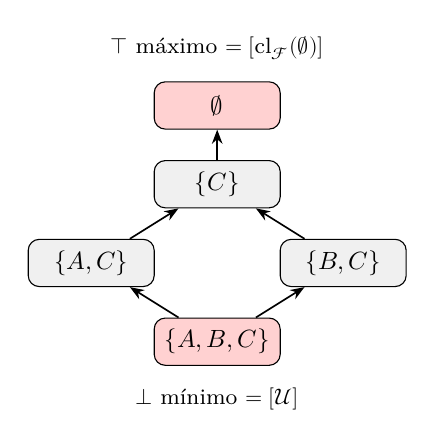
\begin{tikzpicture}[
        cl/.style  = {draw, rounded corners, minimum width=1.6cm, minimum height=0.6cm, font=\small, fill=gray!12},
        ext/.style = {draw, rounded corners, minimum width=1.6cm, minimum height=0.6cm, font=\small, fill=red!18},
        ar/.style  = {-{Stealth[length=1.8mm]}, semithick},
        lbl/.style = {font=\footnotesize}
    ]
        \node[ext] (top) at (0,3)    {$\emptyset$};
        \node[cl]  (C)   at (0,2)    {$\{C\}$};
        \node[cl]  (AC)  at (-1.6,1) {$\{A,C\}$};
        \node[cl]  (BC)  at (1.6,1)  {$\{B,C\}$};
        \node[ext] (bot) at (0,0)    {$\{A,B,C\}$};

        \draw[ar] (bot) -- (AC);
        \draw[ar] (bot) -- (BC);
        \draw[ar] (AC)  -- (C);
        \draw[ar] (BC)  -- (C);
        \draw[ar] (C)   -- (top);

        \node[lbl, above=0.15cm of top] {$\top$ máximo $= [\mathrm{cl}_{\mathcal{F}}(\emptyset)]$};
        \node[lbl, below=0.15cm of bot] {$\bot$ mínimo $= [\mathcal{U}]$};
    \end{tikzpicture}
    \vspace{0.3cm}
\end{frame}

\begin{frame}
    \frametitle{Superclaves y Claves Candidatas}
    \framesubtitle{Definiciones}

    Un subconjunto $K \subseteq \mathcal{U}$ es una \textbf{superclave} si:
    \[ \mathrm{cl}_{\mathcal{F}}(K) = \mathcal{U} \]
    \textit{(Equivalentemente, $[K] = [\mathcal{U}]$ en $\mathbb{T}_{\mathcal{F}}$)}

    \vspace{0.6cm}

    Una \textbf{clave candidata} es una superclave que es mínima bajo inclusión. Es decir, una superclave $K$ tal que:
    \[ \text{No existe un subconjunto propio } K' \subsetneq K \text{ que sea superclave} \]
\end{frame}

\begin{frame}
    \frametitle{Subconjunto Denso y Generador Denso Minimal}
    \framesubtitle{Definiciones}

    \small

    \begin{block}{Subconjunto denso (\textit{dense subset})}
        Un subconjunto $D \subseteq \mathcal{U}$ se llama \textbf{denso} (respecto a $\mathrm{cl}_{\mathcal{F}}$) si:
        \[ \mathrm{cl}_{\mathcal{F}}(D) = \mathcal{U}. \]
    \end{block}

    \begin{block}{Generador denso minimal (\textit{minimal dense generator})}
        Un \textbf{generador denso minimal} es un subconjunto denso que es minimal respecto a la inclusión.
    \end{block}
\end{frame}

\begin{frame}
    \frametitle{Claves como Generadores Topológicos}
    \framesubtitle{Teorema}

    \small

    Sea $(\mathcal{U}, \mathcal{F})$ un esquema relacional finito y sea $\mathbb{T}_{\mathcal{F}}$ su espacio topológico $T_0$ finito asociado. Entonces:

    \vspace{0.3cm}

    \begin{enumerate}
        \item[(i)] Un subconjunto $K \subseteq \mathcal{U}$ es una \textbf{superllave} si y solo si $K$ es \textbf{denso}.

        \vspace{0.2cm}

        \item[(ii)] Un subconjunto $K \subseteq \mathcal{U}$ es una \textbf{clave candidata} si y solo si $K$ es un \textbf{generador denso minimal}.

        \vspace{0.2cm}

        \item[(iii)] Las claves candidatas corresponden exactamente a los \textbf{generadores minimales} del conjunto $\mathrm{cl}_{\mathcal{F}}$-cerrado más grande, $\mathcal{U}$, en el retículo de clausura de $\mathrm{cl}_{\mathcal{F}}$ (es decir, el retículo de subconjuntos $\mathrm{cl}_{\mathcal{F}}$-cerrados de $\mathcal{U}$).
    \end{enumerate}
\end{frame}

\begin{frame}
    \frametitle{Región Cerrada Propia}
    \framesubtitle{Definiciones}
        Un subconjunto $C \subseteq \mathcal{U}$ se llama \textbf{región cerrada propia} si:
        \[ \mathrm{cl}_{\mathcal{F}}(C) = C \qquad \text{y} \qquad C \subsetneq \mathcal{U}. \]
\end{frame}

\begin{frame}
    \frametitle{Generador Propio}
    \framesubtitle{Definiciones}

    Sea $C \subseteq \mathcal{U}$ un conjunto $\mathrm{cl}_{\mathcal{F}}$-cerrado. 
    
    \vspace{0.4cm}
    
    Un subconjunto $X \subseteq \mathcal{U}$ es un \textbf{generador propio} de $C$ si:
    \[ \mathrm{cl}_{\mathcal{F}}(X) = C \quad \text{y} \quad X \subsetneq C \]

\end{frame}

\begin{frame}
    \frametitle{Forma Normal de Boyce-Codd (BCNF)}
    \framesubtitle{Definiciones}

    Un esquema relacional $(\mathcal{U}, \mathcal{F})$ está en \textbf{Forma Normal de Boyce-Codd (BCNF)} si para toda dependencia funcional $X \rightarrow Y$ (con $X, Y \subseteq \mathcal{U}$) tal que:
    \[ Y \subseteq \mathrm{cl}_{\mathcal{F}}(X) \quad \text{y} \quad Y \not\subseteq X \]
    el determinante $X$ es una \textbf{superclave} (es decir, $\mathrm{cl}_{\mathcal{F}}(X) = \mathcal{U}$).
\end{frame} 

\begin{frame}
    \frametitle{Ejemplo: Diagrama de Hasse de $\mathbb{T}_{\mathcal{F}}$ (Arreglado - BCNF)}
    \framesubtitle{$\mathcal{U} = \{A,B,C\}$, \quad $\mathcal{F} = \{A \rightarrow B,\ A \rightarrow C\}$}

    \centering
    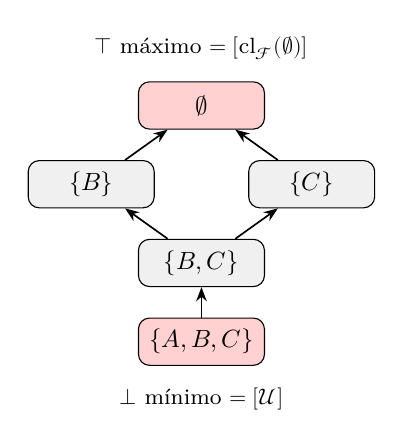
\begin{tikzpicture}[
        cl/.style  = {draw, rounded corners, minimum width=1.6cm, minimum height=0.6cm, font=\small, fill=gray!12},
        ext/.style = {draw, rounded corners, minimum width=1.6cm, minimum height=0.6cm, font=\small, fill=red!18},
        ar/.style  = {-{Stealth[length=1.8mm]}, semithick},
        lbl/.style = {font=\footnotesize}
    ]
        \node[ext] (top) at (0,3)    {$\emptyset$};
        \node[cl]  (B)   at (-1.4,2) {$\{B\}$};
        \node[cl]  (C)   at (1.4,2)  {$\{C\}$};
        \node[cl]  (BC)  at (0,1)    {$\{B,C\}$};
        \node[ext] (bot) at (0,0)    {$\{A,B,C\}$};

        \draw[ar] (bot) -- (BC);
        \draw[ar] (BC)  -- (B);
        \draw[ar] (BC)  -- (C);
        \draw[ar] (B)   -- (top);
        \draw[ar] (C)   -- (top);

        \node[lbl, above=0.15cm of top] {$\top$ máximo $= [\mathrm{cl}_{\mathcal{F}}(\emptyset)]$};
        \node[lbl, below=0.15cm of bot] {$\bot$ mínimo $= [\mathcal{U}]$};
    \end{tikzpicture}
    \vspace{0.3cm}
\end{frame}

\begin{frame}
    \frametitle{Dependencia Multivaluada No Trivial}
    \framesubtitle{Definiciones}

    Una dependencia multivaluada (MVD) $X \twoheadrightarrow Y$ es \textbf{no trivial} si cumple que:
    \[ Y \not\subseteq X \quad \text{y} \quad X \cup Y \neq \mathcal{U} \]
\end{frame}

\begin{frame}
    \frametitle{Rectangularidad sobre un Determinante}
    \framesubtitle{Definiciones}

    Sea $\mathcal{U} = X \sqcup Y \sqcup Z$, y sea $R$ una instancia de relación sobre $\mathcal{U}$. 
    
    \vspace{0.3cm}
    
    Decimos que $R$ es \textbf{rectangular sobre el determinante} $X$ si para todo $x \in \pi_X(R)$, la fibra $R_x := \{(y,z) \mid (x,y,z) \in R\} \subseteq \mathrm{Dom}(Y) \times \mathrm{Dom}(Z)$ satisface:
    \[ R_x = \pi_Y(R_x) \times \pi_Z(R_x) \]

    \vspace{0.3cm}
    
    \textit{Equivalentemente (clausura bajo completación de rectángulos):} \\
    Si $(x, y_1, z_1), (x, y_2, z_2) \in R$, entonces las tuplas mixtas también pertenecen a $R$:
    \[ (x, y_1, z_2), (x, y_2, z_1) \in R \]
\end{frame}

\begin{frame}
    \frametitle{Patrón Rectangular sobre un Ancla}
    \framesubtitle{Definiciones}

    Sea $x \in \mathbb{T}_{\mathcal{F}}$. Un \textbf{patrón rectangular sobre el ancla} $x$ consiste en nodos
    \[ a_1, a_2, b_1, b_2, w_{11}, w_{12}, w_{21}, w_{22} \in \mathbb{T}_{\mathcal{F}} \]
    para los cuales existen representantes
    \[ X, A_1, A_2, B_1, B_2, W_{11}, W_{12}, W_{21}, W_{22} \subseteq \mathcal{U} \]
    tales que:
\end{frame}

\begin{frame}
    \frametitle{Patrón Rectangular sobre un Ancla}
    \framesubtitle{Definiciones}

    \begin{itemize}
        \item[(i)] $[X] = x$, $[A_i] = a_i$, $[B_j] = b_j$, y $[W_{ij}] = w_{ij}$;
        
        \vspace{0.2cm}
        
        \item[(ii)] $X \subsetneq A_i \subseteq W_{ij} \quad \text{para todo } i, j \in \{1, 2\}$;
        
        \vspace{0.2cm}
        
        \item[(iii)] $X \subsetneq B_j \subseteq W_{ij} \quad \text{para todo } i, j \in \{1, 2\}$;
        
        \vspace{0.2cm}
        
        \item[(iv)] los nodos $a_1$ y $a_2$ son incomparables, y los nodos $b_1$ y $b_2$ son incomparables;
        
        \vspace{0.2cm}
        
        \item[(v)] para cada $i, j \in \{1, 2\}$, el nodo $w_{ij}$ se encuentra por encima tanto de $a_i$ como de $b_j$.
    \end{itemize}
\end{frame}

\begin{frame}
    \frametitle{Cuarta Forma Normal (4NF)}
    \framesubtitle{Definiciones}

    Sea $\Sigma$ un conjunto de dependencias (FDs y MVDs) sobre $\mathcal{U}$, y sea $\mathcal{F} \subseteq \Sigma$ el subconjunto de dependencias funcionales.
    
    \vspace{0.4cm}

    Un esquema relacional $(\mathcal{U}, \Sigma)$ está en \textbf{Cuarta Forma Normal (4NF)} si para toda dependencia multivaluada $X \twoheadrightarrow Y$ (con $X, Y \subseteq \mathcal{U}$) tal que:
    \[ \Sigma \vDash X \twoheadrightarrow Y \quad \text{y} \quad Y \not\subseteq X \quad \text{y} \quad X \cup Y \neq \mathcal{U} \]
    el determinante $X$ es una \textbf{superclave}.
\end{frame}

\SlideBackCover{}
\end{document}
